\section{Архитектура решения}
\label{arch}

В этой главе кратко описываются составляющие части решения --- общая схема решения представлена на рисунке~\ref{bl:general}.
Решение состоит из двух частей: модуль трансляции и модуль тестирования трансляции.

\begin{figure}[h!]
  \begin{center}
    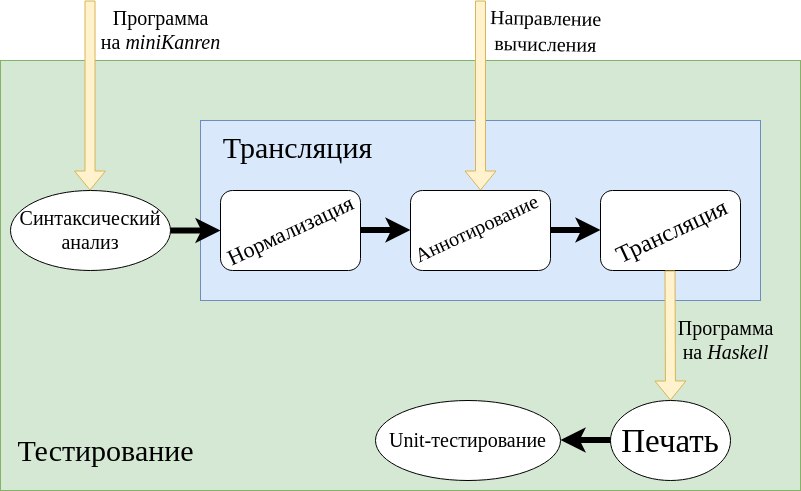
\includegraphics[height=8cm]{figures/diagram.png}
  \end{center}
  \caption{Архитектура решения}
  \label{bl:general}
\end{figure}

Модуль трансляции принимает на вход программу на \miniKanren{} в абстрактном синтаксисе и направление вычисления.
Первый шаг --- нормализация программы на \miniKanren{} (см. раздел~\ref{lab:normform} в главе ~\ref{annotator}).
Затем происходит аннотирования нормализованной программы на \miniKanren{} в абстрактном синтаксисе в соответствии с заданным направлением вычисления (см. главу~\ref{annotator}).
На последнем этапе происходит трансляция нормализованной проаннотированной программы в абстрактном синтаксисе \miniKanren{} в программу в абстрактном синтаксисе \haskell{} (см. главу~\ref{translator}).

Модуль тестирования обсуждается в главе~\ref{test}.
Первый его этап --- синтаксический анализ программы в конкретном синтаксисе \miniKanren{}, в результате которого будет получена программа в абстрактном синтаксисе \miniKanren{}.
Следующий шаг --- запуск модуля трансляции.
Затем происходит трансляция программы в абстрактном синтаксисе языка \haskell{} в программу в конкретном синтаксисе \haskell{}, на рисунке~\ref{bl:general} называемая печатью.
В завершении каждая транслированная программа проходит $unit$-тестирование.

Следующие главы подробно описывают модули решения.

В главе \ref{annotator} описывается разработка алгоритма аннотирования на основе анализа времени связывания.
Вводится понятие нормализованной программы.
Доказывается корректность предложенного алгоритма аннотирования.

Глава \ref{translator} разбирает особенности реляционного языка \miniKanren{} для трансляции, вводит абстрактный синтаксис функционального языка, а также приводит описание шагов трансляции.

Глава \ref{test} посвящена экпериментальному исследованию разработанного алгоритма трансляции из реляционного языка \miniKanren{} в функциональный язык \haskell{}.
В начале предлагается классификация программ на \miniKanren{}, затем описывается система тестирования разработанного транслятора.
В последнем разделе рассматривается результат работы транслятора на более сложном примере --- сортировке.
